%=======================================
%
% $Id$
%
%=======================================

\documentclass[12pt]{article} 
\usepackage{amssymb} 	% additional symbols (there are more packages)
\usepackage{amsmath}
\usepackage{graphicx}
\usepackage{color}

%(Thanks, http://www.terminally-incoherent.com/blog/2007/09/19/latex-squeezing-the-vertical-white-space/)
\usepackage{mdwlist} % for compact lists 

%\usepackage{hyperref}
\usepackage[pagebackref=true,breaklinks=true,letterpaper=true,
colorlinks=true,urlcolor=blue,citecolor=blue,bookmarks=false,
pdfborder={0 0 0}]{hyperref}

\usepackage{anysize} 		% margin package sets tighter margins
\marginsize{1.0in}{1.0in}{0.5in}{1.0in} 	% small margins - left, right, top, bottom

\begin{document}
%\author{Yekaterina Kharitonova}
%\title{Title}
%\maketitle

\hfill Last modified: \today \\%by Yekaterina Kharitonova

\noindent
{\Large \bf Getting started with Bisque}\\ 

This document is intended for users who would like to integrate their analysis code into the Bisque system.
Assuming that you already have that code and the input  required to run it (files and parameters), this overview
outlines steps needed to get started with Bisque~\cite{Bisque}.
%(\url{http://www.bioimage.ucsb.edu/downloads/Bisque%20Database}). 

% -----------------------------------------------
\setcounter{section}{-1} % start the section numbering from 0
\section{Preliminary steps}
\label{sec:Preliminary}
\subsection{iPlant account}
\label{sec:iPlant_account}

Use Trellis~\cite{Trellis}
to create an account and log-in to the dashboard.
One of the services listed under ``Available services" is Bisque.

\begin{figure}[h]
\centering
  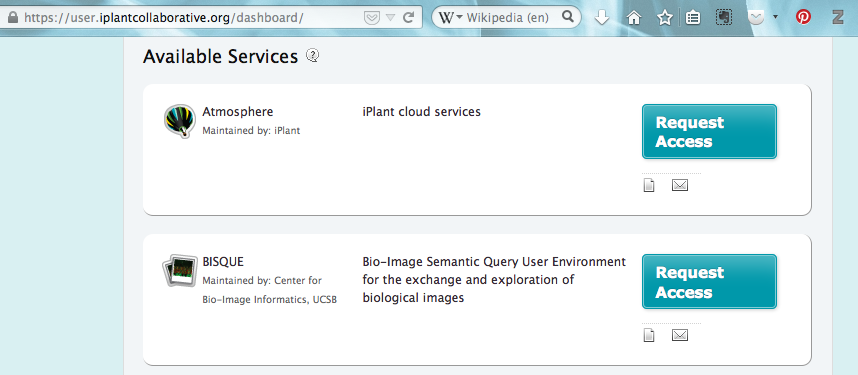
\includegraphics[width=0.6\linewidth]{./figures/available_services.png}
  \label{fig:available_services}
  \caption{The services available through your Trellis dashboard.}
\end{figure}

\begin{figure}[h]
\centering
  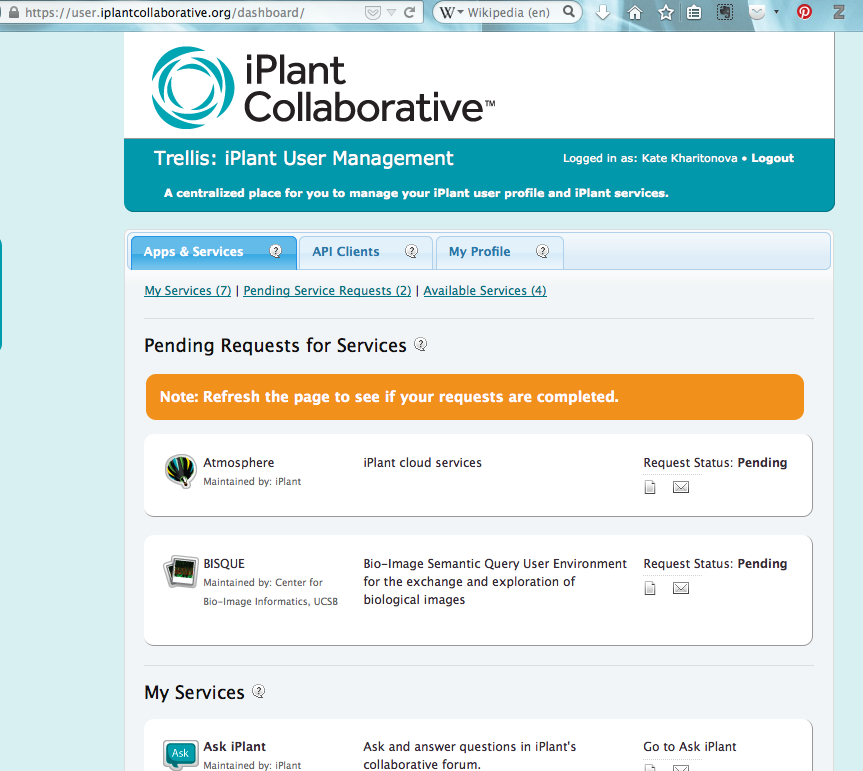
\includegraphics[width=0.6\linewidth]{./figures/pending_request.png}
  \label{fig:pending_request}
  \caption{Pending requests.}
\end{figure}

Once the request is approved, use the 
``Go to BISQUE"~\cite{Bisque-iplant} link to access the 
Bisque database hosted by iPlant (see Fig.\ref{fig:pending_request}).


\subsection{Analysis code}
\label{sec:analysis_code}

Select an existing program to turn into a Bisque module.
This analysis code can be written in any language, and with the help
of the Bisque API, it can be ``wrapped" and connected to the
Bisque services (this is what this tutorial is about).

For the purposes of this tutorial, I am using a C++ program
that finds points of interest in images. 
I created an executable binary, which I can run on the command line.

\begin{verbatim}
./find_points --output-directory=$OUTDIR --has-tip-growth --min-blob-size=5 
--max-blob-size=50 --num-threads=8 $INDAT/Pos001_S001_t%02d_z%02d_ch00.tif
\end{verbatim}

The above command shows the parameters that are required
to run the code, where \texttt{\$OUTDIR} is a variable that holds the path to an output
directory, \texttt{\$INDAT} is a path to where the input files are, 
and \texttt{Pos001\_S001\_t\%02d\_z\%02d\_ch00}
is the Unix printf-style pattern, which describes the format of the 
input file names.
%with the input file names described using a Unix printf-style pattern.

% -----------------------------------------------
\subsection{Overview of steps}
Before we dive in, let's look at a broad picture of the work ahead of us. Don't worry if these steps don't yet make a lot of sense: I will describe each step in more detail in the subsequent sections.

The general idea is this: you have your code that you would like to run using the Bisque system. To do that, you need to describe your module/analysis code to Bisque, i.e. tell Bisque the values for your code's parameters as well as the location/type of the input files. This is taken care of by the module definition XML document. The module definition file describes a web interface that the system will present to you, so that you can set these parameters. You will also need to specify the format/structure and types of the output files in that XML file. %We can think of it as a ``design document" and a ``contract" of sorts. 

The next step is to make sure that your code can talk to the Bisque system. This is accomplished by using the Bisque API~\cite{BisqueAPI}. This API allows you to write what's called  a ``wrapper": a layer of conversion code between your analysis/module code and the Bisque system. It glues together the pieces needed by both layers. Some of its many functions include processing the module definition file, setting up necessary directories, converting data from the Bisque format into the input format expected by your analysis code, running your analysis code and converting the outputs. 

In order to properly test how well your analysis works with Bisque, you need to have access to the Engine Server. The Engine Server is what allows
Bisque to talk to many modules that may exist on many separate machines.
A Bisque package called the Engine Service allows the developers to wrap local files, give them URLs and provide the necessary entry points to facilitate communication between the modules and Bisque. Think of it as a translator that converts text from one language, so that a person who speaks a different language can understand it.

Finally, in order to allow the main Bisque server to access your module, you need to register the Engine Server that's running your module. The registration makes the main Bisque server aware of the existence of your server, and allows them to ``talk" to each other and exchange files.


In summary, below are the steps for setting up a working module taken from the Bisque module creation tutorial~\cite{Bisque-module-creation}:
\begin{enumerate}
\item Creating a module definition XML document
\item Making the module code work with Bisque (either by modifying the module code to use the Bisque API or by writing a wrapper (i.e. conversion glue code))
\item Creating a web server or running the Engine Server
\subitem Engine Service - a configuration file on how the Engine Service will run your code 
\item Registering the module with Bisque 
\end{enumerate}

Let's take a look at each of the steps in more detail.


\section{Creating a module definition XML document}
\label{sec:creating-module-definition-XML}

This section is based on the instructions listed on the Bisque Module Specification page~\cite{Bisque-module-specification}.
After providing an overview of the module system, I outline its various components, constructing an example that uses my analysis code. 
%(see Section~\ref{sec:analysis_code).

\subsection{Module system overview}

The Bisque Module System aims to provide services to the user-created analysis code, so-called analysis module. Every module, before it is used, must be declared to Bisque through module registration. 

To be used with the Bisque system each module must define a module-definition file, which allows the module to be registered. 
Registration involves posting the module definition file to a module manager, %??? 
which can then dispatch execution requests back to the module. The  EngineScripts wraps local scripts and creates a web-service based on module definition file. The EngineServer (installed with Bisque) will manage registration and execution of the local script. It will issue an execution request (MexRequestSpecification), which contains parameters needed to execute the module on behalf of a user. 


\subsection{ Module definition file}

The module-definition file is an XML-encoded file that provides attributes associated with the module. Each module must have a unique name and formally specify its input and output parameters. In addition to input and output, you can specify the coding language, authorship, and code version. 

The module definition document is actually a templated MEX (Module EXecution) document. The template parameters, for example, can be used to render the user interface (UI) for a module if the programmer does not want to fully implement the UI. If, however, the programmer would like to provide a fully customized user interface then the input parameters can be configured to do so. But, let's leave customization for later: it is easiest to start with the automatically provided UI and then customize it if the need arises. 
%On the Bisque Module specification page (http://biodev.ece.ucsb.edu/projects/bisquik/wiki/Developer/ModuleSystem/BisqueModuleSpecification) one can find an example of a module definition file. 

Every module definition file, at a minimum, should specify the following definitions
\begin{itemize}
\setlength{\itemsep}{0.1mm}
\item inputs
\item outputs
\item title
\item description
\item authors
\item thumbnail
\end{itemize}

This means that we can create a bare-bones template (where words in ALL-CAPS are meant to be replaced).
%--- is there another module type other than  type="runtime"?
\begin{verbatim}
<module name="MY_MODULE" type="runtime">
    <tag name="inputs">
    </tag>
    
    <tag name="outputs">
    </tag>

    <tag name="title" value="TITLE" />     
    <tag name="description" value="This module DESCRIPTION" />
    <tag name="authors" value="AUTHORS" /> 
    <tag name="thumbnail" type="file" value="public/thumbnail.png" />
</module>
\end{verbatim}


\subsection{\texttt{inputs} tag}
All input needed by the module has to be declared inside the 
\texttt{<tag name="inputs">}  block (i.e. between the \texttt{<tag ...>} and \texttt{</tag>}). The input can be of the following types:
\begin{itemize*}
\item 
\texttt{system-input}: element required by the module and filled by the system
\item 
\texttt{formal-input}: element required by the module and filled by the UI
\end{itemize*}


\subsubsection{\texttt{system-input} type}
Below is the list of names that are used with the \texttt{system-input} type ((!) indicates a required name):
\begin{itemize*}
\item 
\texttt{mex\_url} (!): a URL pointing to the MEX document; necessary for the module to do anything meaningful
\item 
\texttt{bisque\_token} (!): a token that is used for authentication, without it module can't write anything
\item
\texttt{module\_url}:  a URL to the module % where does it come from?
\end{itemize*}

Now we can add the following required inputs to our module definition file:
\begin{verbatim}
...
    <tag name="inputs">
        <tag name="mex_url"      type="system-input" />
        <tag name="bisque_token" type="system-input" />
    </tag>
...
\end{verbatim}
%Where are the values for e.g. mex_url stored?

\subsubsection{\texttt{formal-input} type}
The formal inputs may be of two ways:
\begin{itemize*}
\item 	a link to an existing resource
\item	a complete resource in-place 
\end{itemize*}

Let's look at them closer.

\subsubsection*{Existing resource}
A link to an existing resource is declared as a tag with a type of a resource you would like to point to. For example, to link to an image
\begin{verbatim}
<tag name="image_url" type="image" />
\end{verbatim}

A link to a resource will get send to the module inside the MEX document looking like this:
\begin{verbatim}
<tag name="image_url" type="image" value="http://host/path" />
\end{verbatim}
%---
%How will it know about the value?
%---
The name here is a user-defined name and will only be used by the module to find the right resource. 
%---
%where does it "find" it?
%---
The type can be any resource type existing in the system. For example you can use: image, dataset or tag. 
%----
%What are the existing resource types other than image, dataset and tag?
%What kind of type is dataset? What's the input -- a collection of files?
%----
Automated interface will try to generate an appropriate resource picker, for example, a browser for an image or a dataset-selection dialog box for a dataset. 
% --- Does it mean that it has to be pre-uploaded?

\subsubsection*{A resource in-place}
Any resource and tag with a non-resource (user-given) type is a resource in-place. They are useful to pass information that should not be stored in the system, such as a numeric parameter or a graphical annotation.
\begin{verbatim}
<tag name="radius" type="number" />
\end{verbatim}

%<tag name="radius" value="6.5" type="number" />
%Note that the above example provides a default value. 
%Obviously these can be templated! I'll describe possible UI configurations in the templating section.
%An in-place resource will be send to the module inside the MEX document looking like this:
%<tag name="radius" value="2.3" type="number" />

Continuing with our analysis code example, we see that our binary takes several input parameters.
\begin{verbatim}
--has-tip-growth 
--min-blob-size=5 
--max-blob-size=50 
--num-threads=8 
$INDAT/Pos001_S001_t%02d_z%02d_ch00.tif
\end{verbatim}

As was described above, our numeric parameters are the ``resource in-place" (the boolean parameter \texttt{--has-tip-growth} can easily be made numeric by using values 1 and 0), and the image input directory is the ``existing resource".
Now we can add them (and their default values) to the inputs tag in our module definition file:
\begin{verbatim}
...
    <tag name="inputs">
        ...
        <tag name="has-tip-growth" value="1" type="number" />
        <tag name="min-blob-size" value="5" type="number" />
        <tag name="max-blob-size" value="50" type="number" />
        <tag name="num-threads" value="8" type="number" />
        
        <tag name="image_url" type="image" />
    </tag>
...
\end{verbatim}


%
%module interface templates vs. resource templates
%
%---
%what are the allowed types of input gobject? point
%polygon
%…
%
%
%---

\section{Making the module code work with Bisque}
\label{sec:making-module-work-with-bisque}



% -----------------------------------------------
{\small
\bibliographystyle{abbrv}
\bibliography{references}
}
\end{document}
